%%%%%%%%%%%%%%%%%%%%%%%%%%%%%%%%%%%%%%%%%
% Journal Article
% LaTeX Template
% Version 1.3 (9/9/13)
%
% This template has been downloaded from:
% http://www.LaTeXTemplates.com
%
% Original author:
% Frits Wenneker (http://www.howtotex.com)
%
% License:
% CC BY-NC-SA 3.0 (http://creativecommons.org/licenses/by-nc-sa/3.0/)
%
%%%%%%%%%%%%%%%%%%%%%%%%%%%%%%%%%%%%%%%%%

%----------------------------------------------------------------------------------------
%	PACKAGES AND OTHER DOCUMENT CONFIGURATIONS
%----------------------------------------------------------------------------------------

\documentclass[twoside]{article}

\usepackage{lipsum} % Package to generate dummy text throughout this template

\usepackage[sc]{mathpazo} % Use the Palatino font
\usepackage[T1]{fontenc} % Use 8-bit encoding that has 256 glyphs
\linespread{1.05} % Line spacing - Palatino needs more space between lines
\usepackage{microtype} % Slightly tweak font spacing for aesthetics
\usepackage{listings}
\usepackage[hmarginratio=1:1,top=32mm,columnsep=20pt]{geometry} % Document margins
\usepackage{multicol} % Used for the two-column layout of the document
\usepackage[hang, small,labelfont=bf,up,textfont=it,up]{caption} % Custom captions under/above floats in tables or figures
\usepackage{booktabs} % Horizontal rules in tables
\usepackage{float} % Required for tables and figures in the multi-column environment - they need to be placed in specific locations with the [H] (e.g. \begin{table}[H])
\usepackage{hyperref} % For hyperlinks in the PDF
\usepackage{graphicx}
\usepackage{lettrine} % The lettrine is the first enlarged letter at the beginning of the text
\usepackage{paralist} % Used for the compactitem environment which makes bullet points with less space between them

\usepackage{abstract} % Allows abstract customization
\renewcommand{\abstractnamefont}{\normalfont\bfseries} % Set the "Abstract" text to bold
\renewcommand{\abstracttextfont}{\normalfont\small\itshape} % Set the abstract itself to small italic text

\usepackage{titlesec} % Allows customization of titles
\renewcommand\thesection{\Roman{section}} % Roman numerals for the sections
\renewcommand\thesubsection{\Roman{subsection}} % Roman numerals for subsections
\titleformat{\section}[block]{\large\scshape\centering}{\thesection.}{1em}{} % Change the look of the section titles
\titleformat{\subsection}[block]{\large}{\thesubsection.}{1em}{} % Change the look of the section titles

\usepackage{fancyhdr} % Headers and footers
\pagestyle{fancy} % All pages have headers and footers
\fancyhead{} % Blank out the default header
\fancyfoot{} % Blank out the default footer
\fancyhead[C]{MiNI - CIBA $\bullet$ November 2015} % Custom header text
\fancyfoot[RO,LE]{\thepage} % Custom footer text

%----------------------------------------------------------------------------------------
%	TITLE SECTION
%----------------------------------------------------------------------------------------

\title{\vspace{-15mm}\fontsize{24pt}{10pt}\selectfont\textbf{High Frequency Trading Price Prediction using LSTM Recursive Neural Networks}} % Article title

\author{
\large
\thanks{Project for Computational Intelligence Business Applications Course}\\[2mm] % Your name
\textsc{Karol Dzitkowski}\\
\normalsize \href{mailto:k.dzitkowski@gmail.com}{k.dzitkowski@gmail.com} \\
\textsc{Tomasz Kozicki}\\
\normalsize \href{mailto:tom.kozicki@o2.pl}{tom.kozicki@o2.pl} \\
\normalsize Warsaw University of Technology\\
\vspace{-5mm}
}
\date{}

%----------------------------------------------------------------------------------------

\begin{document}

\maketitle % Insert title

\thispagestyle{fancy} % All pages have headers and footers

%----------------------------------------------------------------------------------------
%	ABSTRACT
%----------------------------------------------------------------------------------------

\begin{abstract}

The Recurrent Neural Network (RNN) is an extremely powerful model for problems in machine learning that require identifying complex dependencies between temporally distant inputs. It is often used in solving NLP problems, therefore it can be suitable also for stock market prediction. 
In this workwe will try to use recurrent neural network with long short term memory to predict prices in high frequency stock exchange. This paper will show results of implementing such a solution on data from NYSE OpenBook history which allows to recreate the limit order book for any given time.

\end{abstract}

%----------------------------------------------------------------------------------------
%	ARTICLE CONTENTS
%----------------------------------------------------------------------------------------

\begin{multicols}{2} % Two-column layout throughout the main article text

\section{Introduction}

\lettrine[nindent=0em,lines=3]{L} ong Short Memory RNN architecture has been proved to be suprisingly successful in sequence prediction
resolving a problem with vanishing and exploding gradients. In this work we will use Hochreiter \& Schmidhuber (1997) version of LSTM layer. 
The Long Short-Term Memory (LSTM) is a specific RNN architecture whose design makes it much easier to train. While wildly successful in practice, the LSTM's architecture appears to be ad-hoc so it is not clear if it is optimal, and the significance of its individual components is unclear - which was checked by Google in [1]. The aim of this work is to see if the solution will be suitable for predicting prices in stock markets, which are one of the most difficult time series to predict.
Basing on time series data from NYSE OpenBook (which includes every ask and bid prices for one day)
we will try to predict next bid or ask value. If there exist any long or short term dependency with historical data, my LSTM model should outperform
basic perceptron which will be used for comparison. I will also check if changing LSTM model to GRU (Gated Recurrent Unit - Cho et al. 2014.) will
decrease an error rate to establish which solution is best.
All technical implementation will be done in Python using Keras [2] library based on Theano. For performance reasons most computations will be done on GPU using NVIDIA CUDA 7.5 technology. 


%------------------------------------------------

\section{Used method}

In order to gain some persistent knowledge in the network people invented Recurrent Neural Networks which address this issue.
They are networks with loops inside them, allowing information to persist. In that way they are able to learn some long term dependencies between
data in several time points. Usually we consider an unrolled RNN with some length creating chain-like structure.

\begin{figure}[H]
\centering
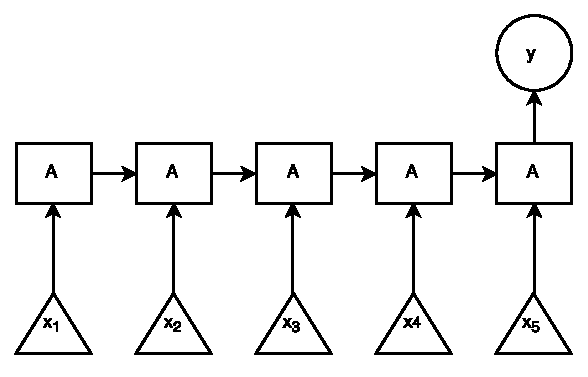
\includegraphics[scale=0.75]{RNN}
\caption{Recursive Neural Network}
\label{ref:rnn}
\end{figure} 

This way they seem to be related to sequences or lists, therefore it will be natural architecture of a network for all time series.
In a normal, basic version the hidden layer \emph{A} is just single \emph{sigmoid} or \emph{tanh} layer.  Due to the fact that for
learning such an architecture uses Backpropagation Through Time (BPTT) it is usually very difficult to train such networks. The problem
is known as vanishing and exploding gradient which makes it impossible for the network to learn long term dependencies. It is solved
by using Long Short Term Memory Networks (LSTM) that handles layer \emph{A} differently. In that model \emph{A} is more complex
structure containing several \emph{tanh} and \emph{sigmoid} layers and \emph{+}, \emph{*} operators.

\begin{figure}[H]
\centering
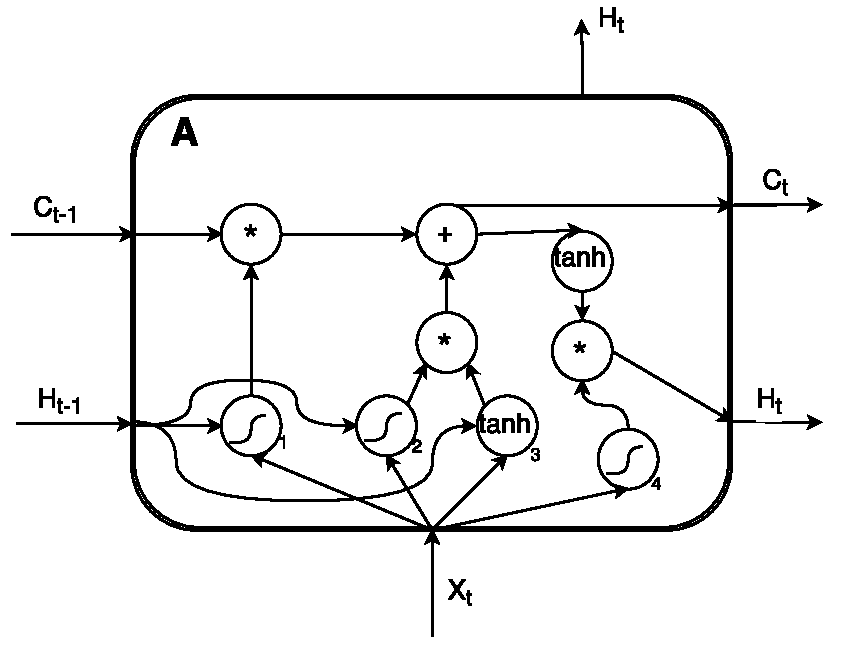
\includegraphics[scale=0.5]{LSTM}
\caption{Recursive Neural Network}
\label{ref:rnn}
\end{figure} 

LSTM handles and passes something called the cell state. It can add or remove information to/from the cell and in that way he stores
historical data. Mathematical definition of that architecture is shown below, where $x_{t}$ is our input, $H_{t-1}$ is the previous output and 
$W_{m}$ are the weights in layer m: \\
\newline
$ \alpha_{t} = \sigma(W_{1} * x_{t} + W_{1} * H_{t-1} + b_{1}) $ \\
$ \beta_{t} = \sigma(W_{2} * x_{t} + W_{2} * H_{t-1} + b_{2}) $ \\
$ \gamma_{t} = tanh(W_{3} * x_{t} + W_{3} * H_{t-1} + b_{3}) $ \\
$ \theta_{t} = \sigma(W_{4} * x_{t} + W_{4} * H_{t-1} + b_{4}) $ \\
\newline
then the new cell state and output are:  \\
\newline
$ C_{t} = \alpha_{t} * C_{t-1} + \beta_{t} * \gamma_{t} $ \\
$ H_{t} = \theta_{t} * tanh(C_{t}) $ \\


Data from NYSE contains information about the symbol of stock, event type, price and volume as well as very precise time to microseconds.
Each record is either bid or ask wchich is indicated by \emph(Side) field of the data.  

\begin{table}[H]
\caption{Selected TAQ NYSE OpenBook Fields}
\centering
\begin{tabular}{ll}
Symbol & Char(11) \\
TradingStatus & Char(1) \\
SourceTime & Int(4) \\
SourceTimeMicroSecs & Int(2) \\
PriceScaleCode & Int(1) \\
PriceNumerator & Int(4) \\
Volume & Int(4) \\ 
Side & Char(1) \\
\end{tabular}
\end{table}

For us the most important are price, volume na side data, because we will use them 
among others as an input to the network. Network will be always trained only for one symbol 
and for events of submission. We are going to experiment with different inputs,
probably using some feature extraction, or choosing custom subset of features by ourselves.
Inputs we are going to consider are:

\begin{itemize}
\item Time - Time since last ask or bid
\item Price - Ask or bid price
\item MidPrice - Difference between highest bid and lowest ask price divided by 2
\item Volume - Volume of last ask or bid
\item Side - Boolean indicating if it was bid or ask
\item PriceDiff - Difference of price between last bid or ask
\end{itemize}

The same inputs will be used to learn ordinary perceptron with one hidden layer. 
Number of nodes in the hidden layer in that \emph(testing) perceptron will be optimized 
to maximize its performance. The problem we want to solve is classification - we want to estimate
if a price (of ask or bid) will be lower, higher or the same in the next transaction. \\
\newline
For the estimation of performance of my neural networks we will use a mean error loss function: \\
\newline
\begin{center}
$ err(t) = \frac{\sum\limits_{i=1}^t (y_{i} \neq Y_{i})}{t - 1} $
\end{center}
%------------------------------------------------

\section{Implementation details}

All development will be done using Python language in version 2.7 using Unix system.
Keras library will be used for development of the solution, since it provides all necessary 
layer types including LSTM in the version described above as well as GRU. Since it uses 
Theano under the hood it is possible to swich on GPU usage, involving that time consuming 
computations will be executed on my NVIDIA graphic card using CUDA technology.

\subsection{Test data providing}
As a basic data that our program operates on we have chosen a NYSE OpenBook Ultra data set from 03/04/2013. The data for given stock symbol is parsed from large binary file and can be conveniently saved to the database and/or file. Then this message book is transformed into an order book message by message to capture the transaction price changes in each moment of time, as well as the history of other stock parameters for further building of the features.

\subsection{Algorithms}
Classes NeuralNetwork and ClassificationPerformance implements:
\begin{itemize} 
\item \emph{Feature selection} \\
A method of performing feature selection with greedy forward selection using cross validation. 
We will try to use only selected features in neural network learning procedure. It gets testing data and neural network in parameters and returns a list of numbers of features to use.
\item \emph{Crossvalidation} \\
A method of using neural network training, cross validating it N times with different test and train data sets randomly choosen from whole dataset. It returns a vector of error rates (training and testing). 
Data is split in proportion defined by a parameter.
\item \emph{T-Student significance test} \\
A method \emph{compare} in ClassificationPerformance class uses t-student distance between error rates
of two different neural networks, and basing on pvalue is states if there exists significant difference 
between two solutions. We will use that to determine if really one neural network performs better than 
the other.
\end{itemize}
%------------------------------------------------

\section{Early Results}
Attached is text file ,,CIBA\_earlyResults.txt'' which contains execution of the program for $19k$ events of the \emph{AIG} stock order book.
Both RNN and MLP report high accuracy from the beginning of iterations. This is very suspicious behaviour that can be explained by the data set characteristics in the next paragraph. As we can see the cross validation correctly divides the samples for training and testing and the feature selection chooses the best features. Due to no negligible differences in performance the program reports that RNN and MLP are not significantly different.

\subsection{Imbalanced data set}
The problem that occurred during test phase turned out to be originating with data approach.
As the response value for our vector of features we have choosen indicator wheter the transaction price for a given stock has dropped, stayed the same or risen. This results in response variable being mainly dominated by the second case, because transactions on NYSE OpenBook occur much less often than we initialy expected, making below around 10 percent of overall entries.
Above leads to the poor learning performance of the neural networks. It is just easier for them to assume no transaction price change since it is the correct choice most of the time.

\section{Reviewed solution}

Because we did not get satisfactory results, we had to change our solution in case of features and
balance of classes in our data. Ultimately we got balanced data and many more features, and better results.
Below we exmplain detailed final solution:

\subsection{Data set}

As message book in it's raw form yields little indication of transaction price changes there is need to convert it into more structured form. The representative structure  that represents prices and volumes on both buyers and sellers side is called order book.
Each event from the message book regarding analyzed stock symbol is compared with existing order book records. These are grouped into two lists: bid side and ask side. The bid side is sorted descending by price and at each price level contains the accumulated volume information. The ask side is sorted ascending by price and at each price level contains the accumulated volume information. Whether it is buy or sell order it is checked if the price allows for a transaction to take place. If so the current transaction price is updated while previous transaction price still being held for comparison. Otherwise this message is added to appropriate record in order book with matching price (total volume is incremented).

TUTAJ OPISZ JAK TWORZYSZ ORDER BOOKA I JAKIE FEATURES Z NIEGO BIERZESZ
ROWNIEZ OPISZ JAKIE TERAZ MAMY KLASY CZYLI CO ZNACZA - CZYLI JAK ZMIENIL SIE OUTPUT, CZYM JEST TEN PRICE
NASTEPNIE NAPISZ JAK ZALEZY ILOSC FEATURES OD LEVEL I ZE MOZNA GO USTAWIAC

TUTAJ OPISZ JAK BALANSUJESZ DANE - ZE ROBISZ UNDERSAMPLING - OPISZ TEN ALGORYTM TROCHE MOZE?

\subsection{Features and output}
We identify a collection of proposed attributes that are divided into two categories: basic and time-insensitive, all of which can be directly computed from the data. Attributes in the basic set (v1) are the prices and volumes at both ask and bid sides up to n different levels (that is, price levels in the order book at a given moment), which can be directly fetched from the order book. Attributes in the time-insensitive set are easily computed from the basic set at a single point in time. Of this, bid-ask spread and mid-price, price ranges, as well as average price and volume at different price levels are calculated in feature sets v2, v3, and v4, respectively; while v5 is designed to track the accumulated differences of price and volume between ask and bid sides.

With each new message arriving to the order book the history of features and output is appended with new set of those.
The response variable is a category number indicating whether the transaction price for a given stock has dropped, stayed the same or risen in the next moment.

NAPISZ ZE UZYWALISMY FEATURE SELECTION ALE WYSZLO NAM ZE WSZYSTKIE SA TAK SAMO WAZNE PRAWIE I TUTAJ JAKO
GLUPI DOWOD DAMY TEN WYKRESIK:

As the number of features rises with incremented level we considered that it may be beneficial for computation time to select features which are most important. If a number of them would stand out in terms of effect on accuracy then it would be wise to choose thiem as a best subset for training.
To evaluate this aspect we used mentioned feature selection algorithm. For this the initial feature set based on level equal to 3 was determined to 30. As it turned out there is no significant difference in impact of features on accuracy which is shown on the barplot below. Therefore we decided to conduct the fiinal evaluation on all initial features.

\begin{figure}[H]
\centering
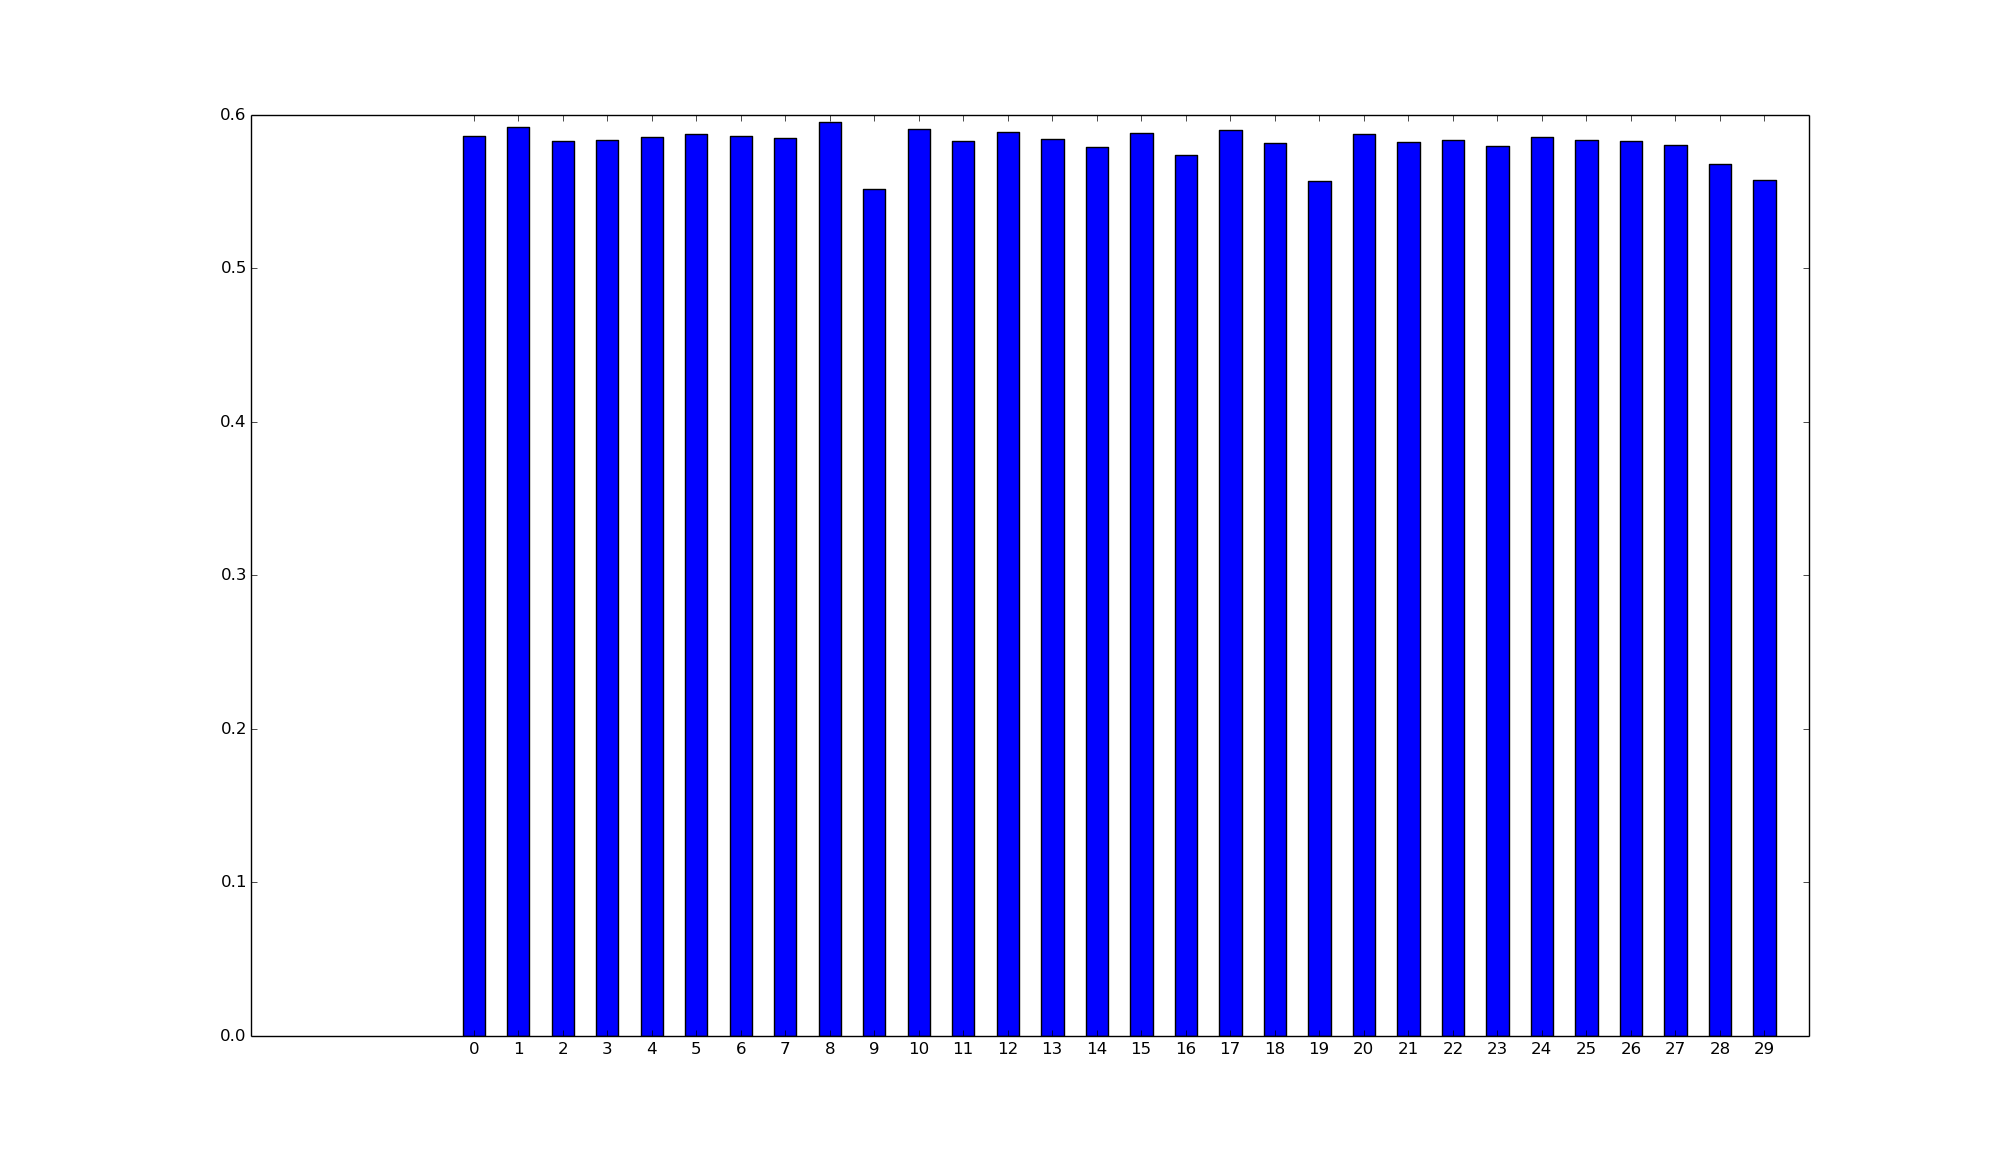
\includegraphics[scale=0.15]{../results/features}
\caption{Features importance}
\label{ref:rnn}
\end{figure} 

\subsection{Input and output form}
Each training record passed to neural network consists of n consecutive records from order book history. Each of this records consists of all feature values and response variable.

\subsection{Networks}
At the end we resigned from using GRU network and instead focused on LSTM, comparing it to ordinary MLP.
For learning we used Stochastic gradient descent optimizer with categorical crossentropy loss function.
Below we present actual models of networks used:
\begin{lstlisting}[language=Python, frame=single, basicstyle=\tiny]
PERCEPTRON:
model = Sequential()
model.add(TimeDistributedDense(output_dim=self.hidden_cnt,
                               input_dim=self.input_dim,
                               input_length=self.input_length,
                               activation='sigmoid'))
model.add(TimeDistributedMerge(mode='ave'))
model.add(Dropout(0.5))
model.add(Dense(self.hidden_cnt, activation='tanh'))
model.add(Dense(self.output_dim, activation='softmax'))

LSTM:
model = Sequential()
model.add(LSTM(output_dim=self.hidden_cnt,
			   input_dim=self.input_dim,
			   input_length=self.input_length,
			   return_sequences=False))
model.add(Dropout(0.5))
model.add(Dense(self.hidden_cnt, activation='tanh'))
model.add(Dense(self.output_dim, activation='softmax'))
\end{lstlisting}

\subsection{GPU usage}
Because of the fact that our NN are learning slowly and teaching them is time consuming we found
useful to switch on BLAS and CUDA enabled devices usage by Theano library. To do that it was sufficient to
create a file ~/.theanorc with content: \\
\begin{lstlisting}
[global]
floatX = float32
device = gpu1

[blas]
ldflags = -L/usr/local/lib -lopenblas

[nvcc]
fastmath = True
\end{lstlisting}

Using that new architecture and solution we received our final results.

\section{Final Results}

As the test data we have chosen AIG order book generated by analysing 2 milion records from NYSE OpenBook. This yielded in balanced test data set in size of ~33k.
\newline
33120 Total records including: \\
11040.0 records with price down \\
11040.0 records with price stable \\
11040.0 records with price up \\

A POTEM CO DOSTALISMY: \\
\newline
\begin{lstlisting}[caption={RNN vs MLP with 200 epochs and 20 crossvalidation steps output:}]
RNN is significantly better than MLP
RNN avg err = 0.567300724638, 
MLP avg err = 0.600966183575
\end{lstlisting}

\begin{figure}[H]
\centering
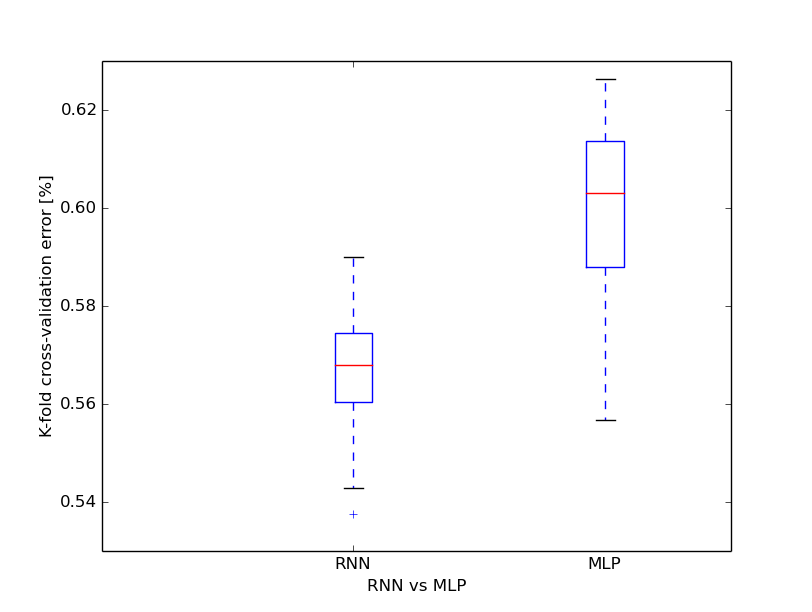
\includegraphics[scale=0.4]{../results/rnn_vs_mlp_200iters_20cross}
\caption{Features importance}
\label{ref:rnn}
\end{figure} 

TUTAJ TRZEBA POZBIERAC NASZE OSTATECZNE WYNIKI, CO NAM WYSZLO, NASZE WYKRESY

\section{Conclusion}

KROTKIE PODSUMOWANIE TEGO CZEGO SIE NAUCZYLISMY I CO NAM WYSZLO Z NASZEGO REASERCHU

%----------------------------------------------------------------------------------------
%	REFERENCE LIST
%----------------------------------------------------------------------------------------

\begin{thebibliography}{99}

\bibitem{art01}
    ``Modeling high-frequency limit order book dynamics with support vector machines'' \\
\emph{http://www.math.fsu.edu/~aluffi/archive/paper462.pdf} \\
	Alec N. Kercheval and Yuan Zhang, 24 October 2013

\bibitem{art02}
	``An Empirical Exploration of Recurrent Network Architectures'' \\
\emph{http://jmlr.org/proceedings/papers/v37/jozefowicz15.pdf}
	Rafal Jozefowicz, Wojciech Zaremba, Ilya Sutskever
	
\bibitem{art03}
	``Long short-term memory'' \\
\emph{http://deeplearning.cs.cmu.edu/pdfs/Hochreiter97\_lstm.pdf}
	Sepp Hochreiter and Jurgen Schmidhuber, 1997

\bibitem{tut01}
    ``LSTM implementation explained'' \\
\emph{https://apaszke.github.io/lstm-explained.html} 
	Adam Paszke, 30 Aug 2015

\bibitem{tut02}
    ``Recurrent Neural Networks Tutorial - Implementing a RNN with Python, Numpy and Theano'' \\ \emph{http://www.wildml.com/2015/09/recurrent-neural-networks-tutorial-part-2-implementing-a-language-model-rnn-with-python-numpy-and-theano/}

\bibitem{tut03}
    ``Keras library'' \\
\emph{http://keras.io}

\bibitem{tut04}
    ``Supervised Sequence Labelling with Recurrent Neural Networks''	\\	\emph{http://www.cs.toronto.edu/~graves/preprint.pdf} 
    Alex Graves

\end{thebibliography}

%----------------------------------------------------------------------------------------

\end{multicols}

\end{document}
